\documentclass[compress]{beamer}

\usetheme{Hamburg}

\usepackage[T1]{fontenc}
\usepackage[utf8]{inputenc}

\usepackage{lmodern}

\usepackage[english]{babel}
%\usepackage[ngerman]{babel}

\usepackage{eurosym}
\usepackage{listings}
\usepackage{microtype}
\usepackage{units}
\usepackage{hyperref}
\usepackage{url}


\lstset{
	basicstyle=\ttfamily\footnotesize,
	frame=single,
	numbers=left,
	language=C,
	breaklines=true,
	breakatwhitespace=true,
	postbreak=\hbox{$\hookrightarrow$ },
	showstringspaces=false,
	tabsize=4,
	captionpos=b,
	morekeywords={gboolean,gpointer,gconstpointer,gchar,guchar,gint,guint,gshort,gushort,glong,gulong,gint8,guint8,gint16,guint16,gint32,guint32,gint64,guint64,gfloat,gdouble,gsize,gssize,goffset,gintptr,guintptr,int8_t,uint8_t,int16_t,uint16_t,int32_t,uint32_t,int64_t,uint64_t,size_t,ssize_t,off_t,intptr_t,uintptr_t,mode_t}
}

\title{I/O analysis of climate applications}
\author{Arne Beer \& Frank Röder}
\institute{Arbeitsbereich Wissenschaftliches Rechnen\\Fachbereich Informatik\\Fakultät für Mathematik, Informatik und Naturwissenschaften\\Universität Hamburg}
\date{$\text{2016-09-01}^{\text{st}}$}

\titlegraphic{
\includegraphics[width=0.75\textwidth]{gfx/logo}}

\begin{document}

\begin{frame}
	\titlepage
\end{frame}

\begin{frame}
	\frametitle{Content (Agenda)}

	\tableofcontents[hidesubsections]
\end{frame}

\section{Introduction}
\begin{frame}
	\frametitle{Introduction}
\begin{itemize}
	\item what climate models do
	\item what is important about them
	\item take a look at the workflow (pre-/post-processing)
	\item take a look at storage systems
\end{itemize}

\end{frame}

\subsection{Goals and Tasks}
\begin{frame}
	\frametitle{discover applications of climate system}

\begin{itemize}
	\item run simulations of related models
	\item analyze their input and output
	\item take a look at the life-cycle of data
	\item deliver knowledge about that
\end{itemize}

\end{frame}

\section{Models and Research}
\begin{frame}
    \frametitle{Considered Climate Models}

    \begin{itemize}
    	\item IFS (Integrated Forecasting System)
	\item AWIPS II (Advanced Weather Interactive Processing System II)
	\begin{itemize}
	    \item EDEX (Environmental Data EXchange)
	    \item CAVE (Common AWIPS Visualization Environment)
	\end{itemize}
	\item CESM (Community Earth System Model)
	\item ECOHAM5 (ECOsystem Model Hamburg Version 5)
    \end{itemize}

\end{frame}

\subsection{IFS}
\begin{frame}
	\frametitle{IFS}
	\begin{itemize}
	    \item provides OpenIFS \cite{ifs}
	    \item global weather forecasting
	    \item biospheric and hydrological processes
	    \item ocean wave, ocean, sea ice
		\item well documented and maintained model
		\item license forbids benchmarking
	\end{itemize}
\end{frame}

\subsection{Awips II}
\begin{frame}
    \frametitle{Awips II}
    \begin{center}
    	\begin{figure}
			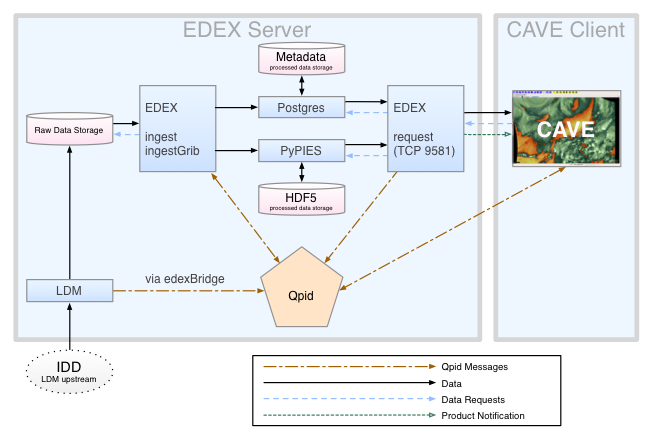
\includegraphics[width=0.85\textwidth]{gfx/awipsII.png}
      	  	\caption[]{Awips Infrastructure \cite{Uni01}}
		\end{figure}
	\end{center}
\end{frame}

\subsection{CAVE}
\begin{frame}
    \frametitle{CAVE}

    \begin{itemize}
        \item data analysis and manipulation \cite{AwipsDocs}
        \item layer different scenarios (multiple radars in hdf5)
	\end{itemize}

    \begin{center}
    	\begin{figure}
			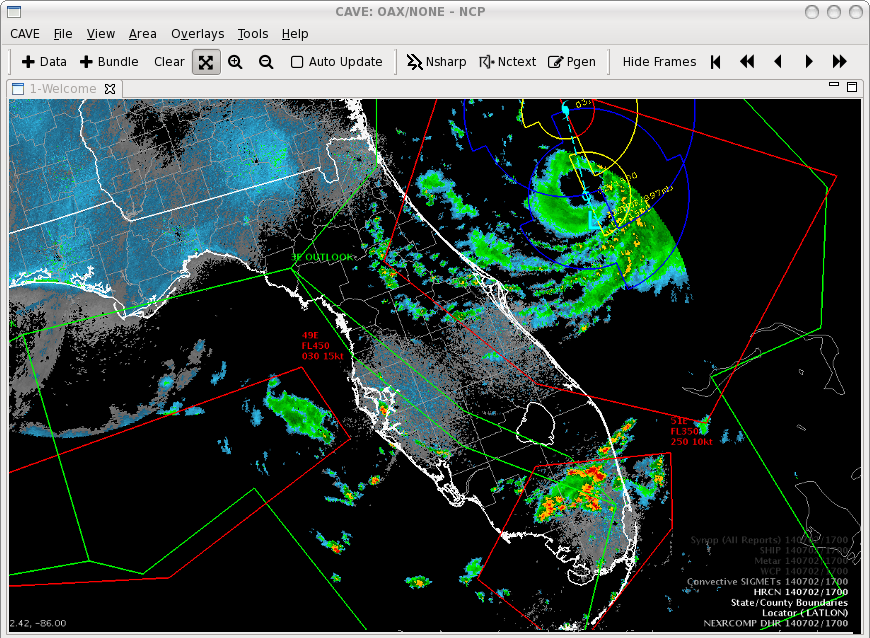
\includegraphics[width=0.64\textwidth]{gfx/Unidata_AWIPS2_CAVE.png}
      	  	\caption[]{Awips Infrastructure \cite{Uni01}}
		\end{figure}
	\end{center}
\end{frame}


\subsection{CESM}
\begin{frame}
    \frametitle{CESM}
    	\begin{itemize}
    	    \item Community Earth System Model
			\item model for global climate simulation
			\item covers atmosphere, land, land ice, sea ice, ocean and river
			\item provides scripts for setting up the machine in 4 commands
		    \item good configurability with xml files
		    \item requires netCDF format for input data \cite{CESMDocs}
		\end{itemize}
\end{frame}

\begin{frame}
    \frametitle{CESM Failure}
    	\begin{itemize}
		    \item fixed Broken setup scripts
		    \item fails during compilation
		    \begin{itemize}
		        \item parallel IO library
		    \end{itemize}
		    \item no documentation
		\end{itemize}
\end{frame}

\subsection{ECOHAM5}
\begin{frame}
	\frametitle{ECOHAM5}
	\begin{itemize}
		\item model for atmospheric circulation with focus on the nord sea \cite{echam}
        \item a progression of older models by using MPI
	\end{itemize}
\end{frame}

\begin{frame}
	\frametitle{ECOHAM5 research status}
	\begin{itemize}
		\item access granted two weeks ago
		\item setup and compilation is very easy
		\item running on cluster
		\item no results due to limited time in exam period
	\end{itemize}
\end{frame}

\subsection{Input and Output analysis}
\begin{frame}[fragile]
	\frametitle{I/O analysis}
	\begin{center}
	\begin{figure}
	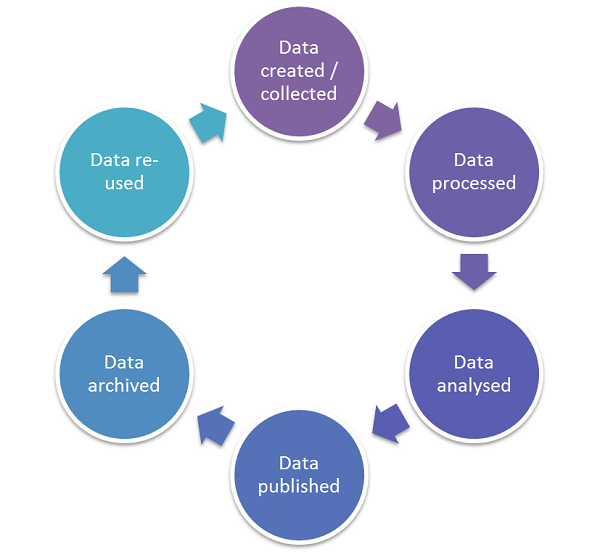
\includegraphics[width=0.6\textwidth]{gfx/DataLifecycle.png}
	\caption[]{Data Life-Cycle \cite{LanUni}}
	\end{figure}
	\end{center}

\end{frame}


\section{Summary}

\begin{frame}
	\frametitle{Summary}

	\begin{itemize}
		\item climate models
		\begin{itemize}
			\item CESM, ECOHAM5
			\item original research goal failed.
			\item investigation of different models
		\end{itemize}

		\item analyzing of weather
		\begin{itemize}
		    \item AWIPS II
		\end{itemize}
	\end{itemize}
\end{frame}

\section*{Literature}

\begin{frame}[allowframebreaks]
	\frametitle{Literature}
    \frametitle{Sources}

	\bibliographystyle{alpha}
	\bibliography{literatur.bib}
\end{frame}

\end{document}
